\chapter{Modelado de escenarios}
A continuacion presentaremos diversos escenarios que permiten lograr un modelado del sistema basado en interacciones

\section{Ingreso de un pedido}
%TODO: escenario uno, ingresa un pedido de solo bebidas
Como primer escenario mostraremos lo que ocurre cuando ingresa un pedido al sistema y este esta formado por solo bebidas. En este caso el pedido va ser creado  y luego el contralador de preingreso se encargar� de pasarselo al manejador de listos, ya que no hay nada que hacer con este pedido. Vamos a suponer por simplicidad que el pedido esta formado por una gaseosa y una cerveza. Asumimos tambi�n en este escenario que el cliente ya se valido (o es NULL si es un pedido de cliente anonimo) y que hay stock sufiencte para armar el pedido.

En este escenario ademas no modelamos todo el proceso de creaci�n de un pedido, el cual ser� desarrollado posteriormente

Veamos el diagrama de secuencias relativo al escenario:
%\begin{landscape}
\begin{figure}[H]
\centering
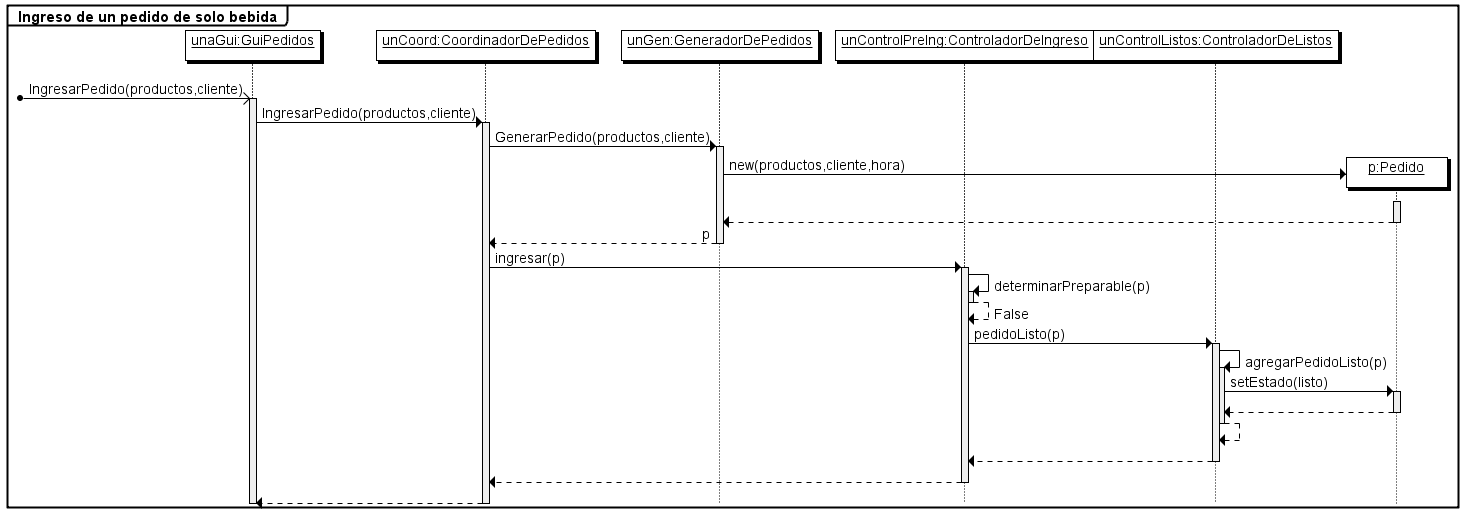
\includegraphics[scale=0.32]{./figuras/ingresaBebida.png}
\end{figure}
%\end{landscape}

%TODO: dos, ingresa un pedido de pizzas solamente y hay cosas en la cola de ingreso

%TODO: ingresa un pedido mixto y queda en la cola de listos, tener en cuenta q la seleccion de horno se hace mientras es intentna ingresar

%TODO: generacion de un pedido

\section{Iniciar sesion de cliente}

\section{aviso de stock critico}

%TODO: no hay suficiente relleno de una empanada y de una pizza

\section{modificacion de la cola de pedidos}

%TODO: mover un pedido un lugar hacia arriba y otro hacia abajo

\section{Preparacion de pedidos}

%TODO: ingresa un pedido y no hay nada esperando preparandose tonces pasa a preparse

%TODO: se empieza a preparar un pedido mixto de la cola de ingreso

%TODO: maestro pide pedido a preparar y se le da un pedido que el otro maestro esta preparando

\section{Cocci�n de pedidos}

%TODO: se termina de prepara un pedido y no hay nada esperando

%TODO: se termina de prepara un pedido y se encola en su horno

%TODO: se termina de cocinar algo en un modulo agil y se toma un pedido chico

%TODO: se termina de cocinar algo en un modulo normal y se toma un pedido normal

%TODO: se termina de cocinar algo en un modulo y no hay nada a continuaci�n

%TODO: se saca un producto y se termino de cocinar

\section{Despachar pedido}

%TODO: se despacha un pedido remoto

%TODO: se despacha un pedido local

\section{Se cierra una mesa}

%TODO: se cierra una mesa y se registra la forma de pago

\section{Cancelacion}

%TODO: todos los escenarios de cancelacion

\section{Actualizar precios}
La actualizacion de los precios de pedidos se realiza de la siguiente manera. Al abrirse la pantalla de ABM de productos, se cargan todos los productos en pantalla. Luego se puede elegir un producto de la lista y un nuevo valor para el precio.

Vamos a modelar el escenario donde se cambia el precio de la pizza de muzzarella a \$30.

Notar que probablemente la GUI realice operaciones con la lista de productos que obtiene, por ejemplo cargar una lista en pantalla para mostrar los pedidos, etc. Sin embargo consideramos que los aspectos propios de la GUI no entran en lo que se debe modelar en este trabajo.

\begin{figure}[H]
\centering
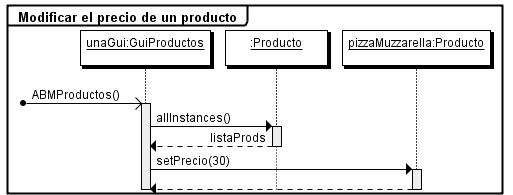
\includegraphics[scale=0.7]{./figuras/modifPrecio.png}
\end{figure}


\section{Consulta de estado de pedido}
El escenario a modelar es el siguiente: El encargado de pedidos abre la gui para consultar el estado de un pedido, entonces la gui muestra los pedidos y cuando el encargado encuentra el que busca, pide ver el estado. El coordinador es el encargado de hacer de adaptador entre la GUI y los pedidos.

En el diagrama suponemos que se llama un metodo de la gui verEstado, esto en verdad es abrir la interfaz para ver los estados de pedidos, es decir no es un metodo como tal, pero sirve para dar idea de que alguien le dice a la GUI que busque los pedidos y consulte el estado.

\begin{figure}[H]
\centering
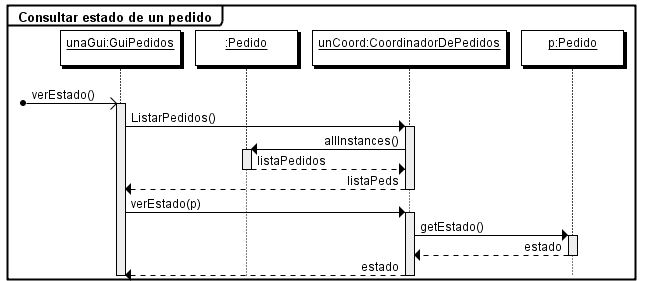
\includegraphics[scale=0.7]{./figuras/verEstado.png}
\end{figure}


